% !TEX root = paper.tex
% !TEX encoding = UTF-8 Unicode
% -*- coding: UTF-8; -*-
% vim: set fenc=utf-8
% !TEX spellcheck = en-US
\section{Results}
\label{sec:results}

%------------------------------%
%: see Figure~\ref{fig:results}
\begin{figure}%[!ht]%%[p!]
\centering{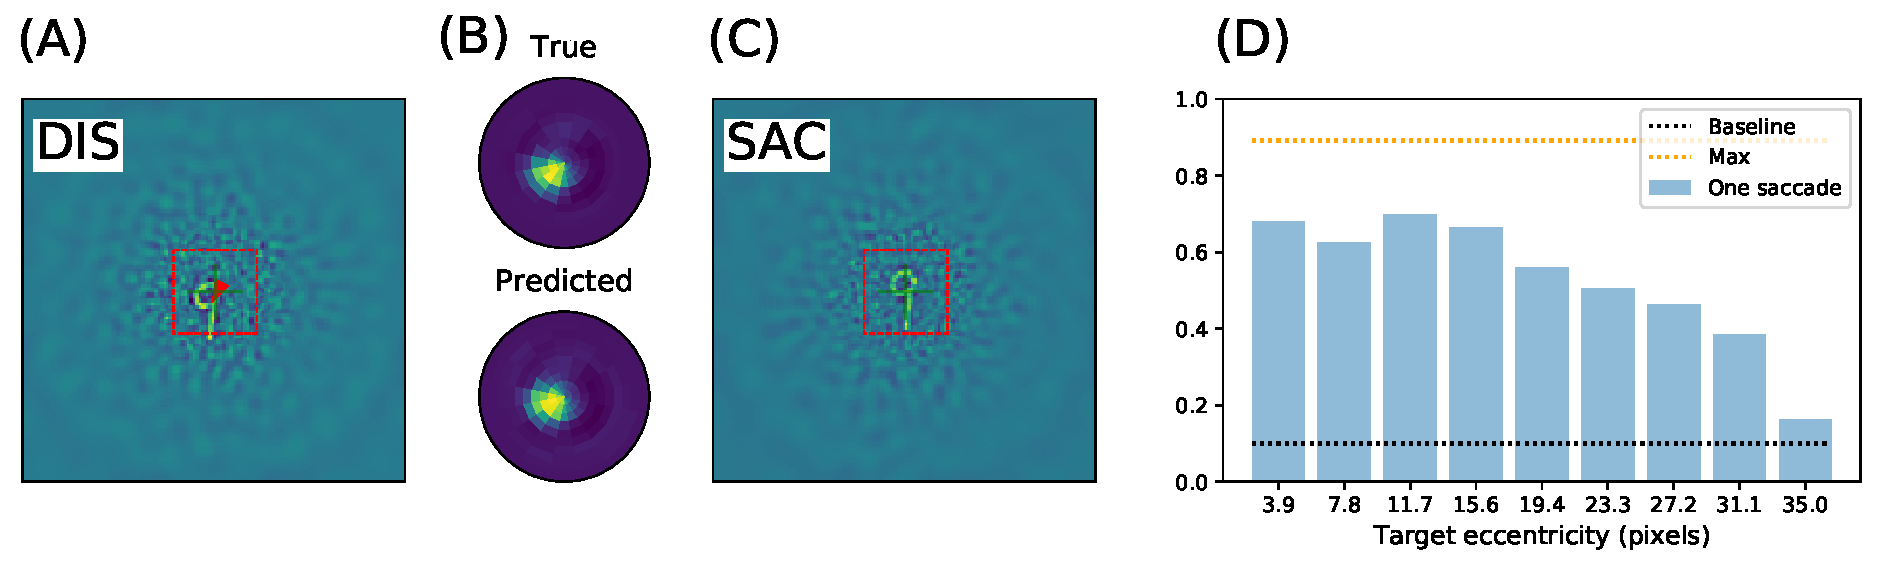
\includegraphics[width=\linewidth]{fig_result}}
\caption{
{\bf Results}: Results from simulations of the active vision agent.
(A)~The input image ('DIS', see  Figure~\ref{fig:results}-C)  is transformed into a retinotopic representation which is used as the input to the 'Where' pathway of the agent. This pathway is a function that transforms this retinal image into a map predicting (B)~the accuracy of a classification in the 'What' pathway. The network fitting for this function is trained in a supervised using a ground truth ('True') and we show here a prototypical example of the 'Predicted' map. This allows to (C)~generate a saccade to the most likely position in visual space to achieve a successful classification. (D)~Testing over a range of $XXX$ different trials (different positions and digits), we show here the final average classification accuracy as a function of eccentricity. This shows first the results of the 'What' pathway ('No saccade') which quickly drops to baseline level after 3 scales. Second, we show the accuracy results obtained after one saccade which now drops to 'baseline' after 7 scales. This shows that by performing only one saccade, the image is now partly covered.
\label{fig:results}}%
\end{figure}%
%%------------------------------%
%result

 In particular, this shows that

% energy consumption


% inhibition of return
